\documentclass[10pt,twocolumn]{article}

% use the oxycomps style file
\usepackage{oxycomps}
\usepackage{amsmath}
\usepackage{graphicx}
\usepackage{subcaption}

% usage: \fixme[comments describing issue]{text to be fixed}
% define \fixme as not doing anything special
\newcommand{\fixme}[2][]{#2}
% overwrite it so it shows up as red
\renewcommand{\fixme}[2][]{\textcolor{red}{#2}}
% overwrite it again so related text shows as footnotes
%\renewcommand{\fixme}[2][]{\textcolor{red}{#2\footnote{#1}}}

% read references.bib for the bibtex data
\bibliography{bibliography}

% include metadata in the generated pdf file
\pdfinfo{
    /Title (Lit Review)
    /Author (Ryan Morrell)
}

% set the title and author information
\title{Procedural Animation of Humanoid Bodies with Inverse Kinematics}
\author{Ryan Morrell}
\affiliation{Occidental College}
\email{rmorrell@oxy.edu}

\begin{document}

\maketitle

\section{Introduction}
Traditional 3D animation techniques create motion by interpolating a system of joints and bones through a series of predefined positions called keyframes. This technique has been used for decades but in 3D animation for movies, games, and other digital media its slow methodical nature can be a major drawback. Inverse kinematics is a family of algorithms that animates joint structures procedurally, saving time while preserving authentic movements and allowing animations to adapt to changing conditions in the animation environment.

Game developers use inverse kinematics to create flexible and responsive character animators with believable movement across any number of unpredictable scenarios \cite{litReview}\cite{ShadowofC}. This can be incredibly useful for smaller game development teams. Traditional key-frame animation requires preparing and recording every necessary permutation of each animated action before runtime. As such, animators must be exhaustive in order to produce quality results. Using Inverse kinematics, a single reactive skeleton can be programmed to generate new animations as needed with only a few adaptive targets as input\cite{UnchartedClimbing}\cite{uncharted}.

Forwards And Backwards Inverse Kinematics, better known as FABRIK, is an iterative inverse kinematics solver that animates skeletal structures by pushing and pulling a chain of joints between a target and a root position. FABRIK is quick enough to be run in real time and effective enough to create realistic humanoid poses. Its lightweight implementation and simple tactics for manipulation make it ideal for the 3D media creation \cite{litReview}. In this paper FABRIK is used to create a semi-realistic humanoid skeleton in the Unity game engine that can recreate detailed motion capture animations from a small set of targets.

\begin{figure}[h]
\centering
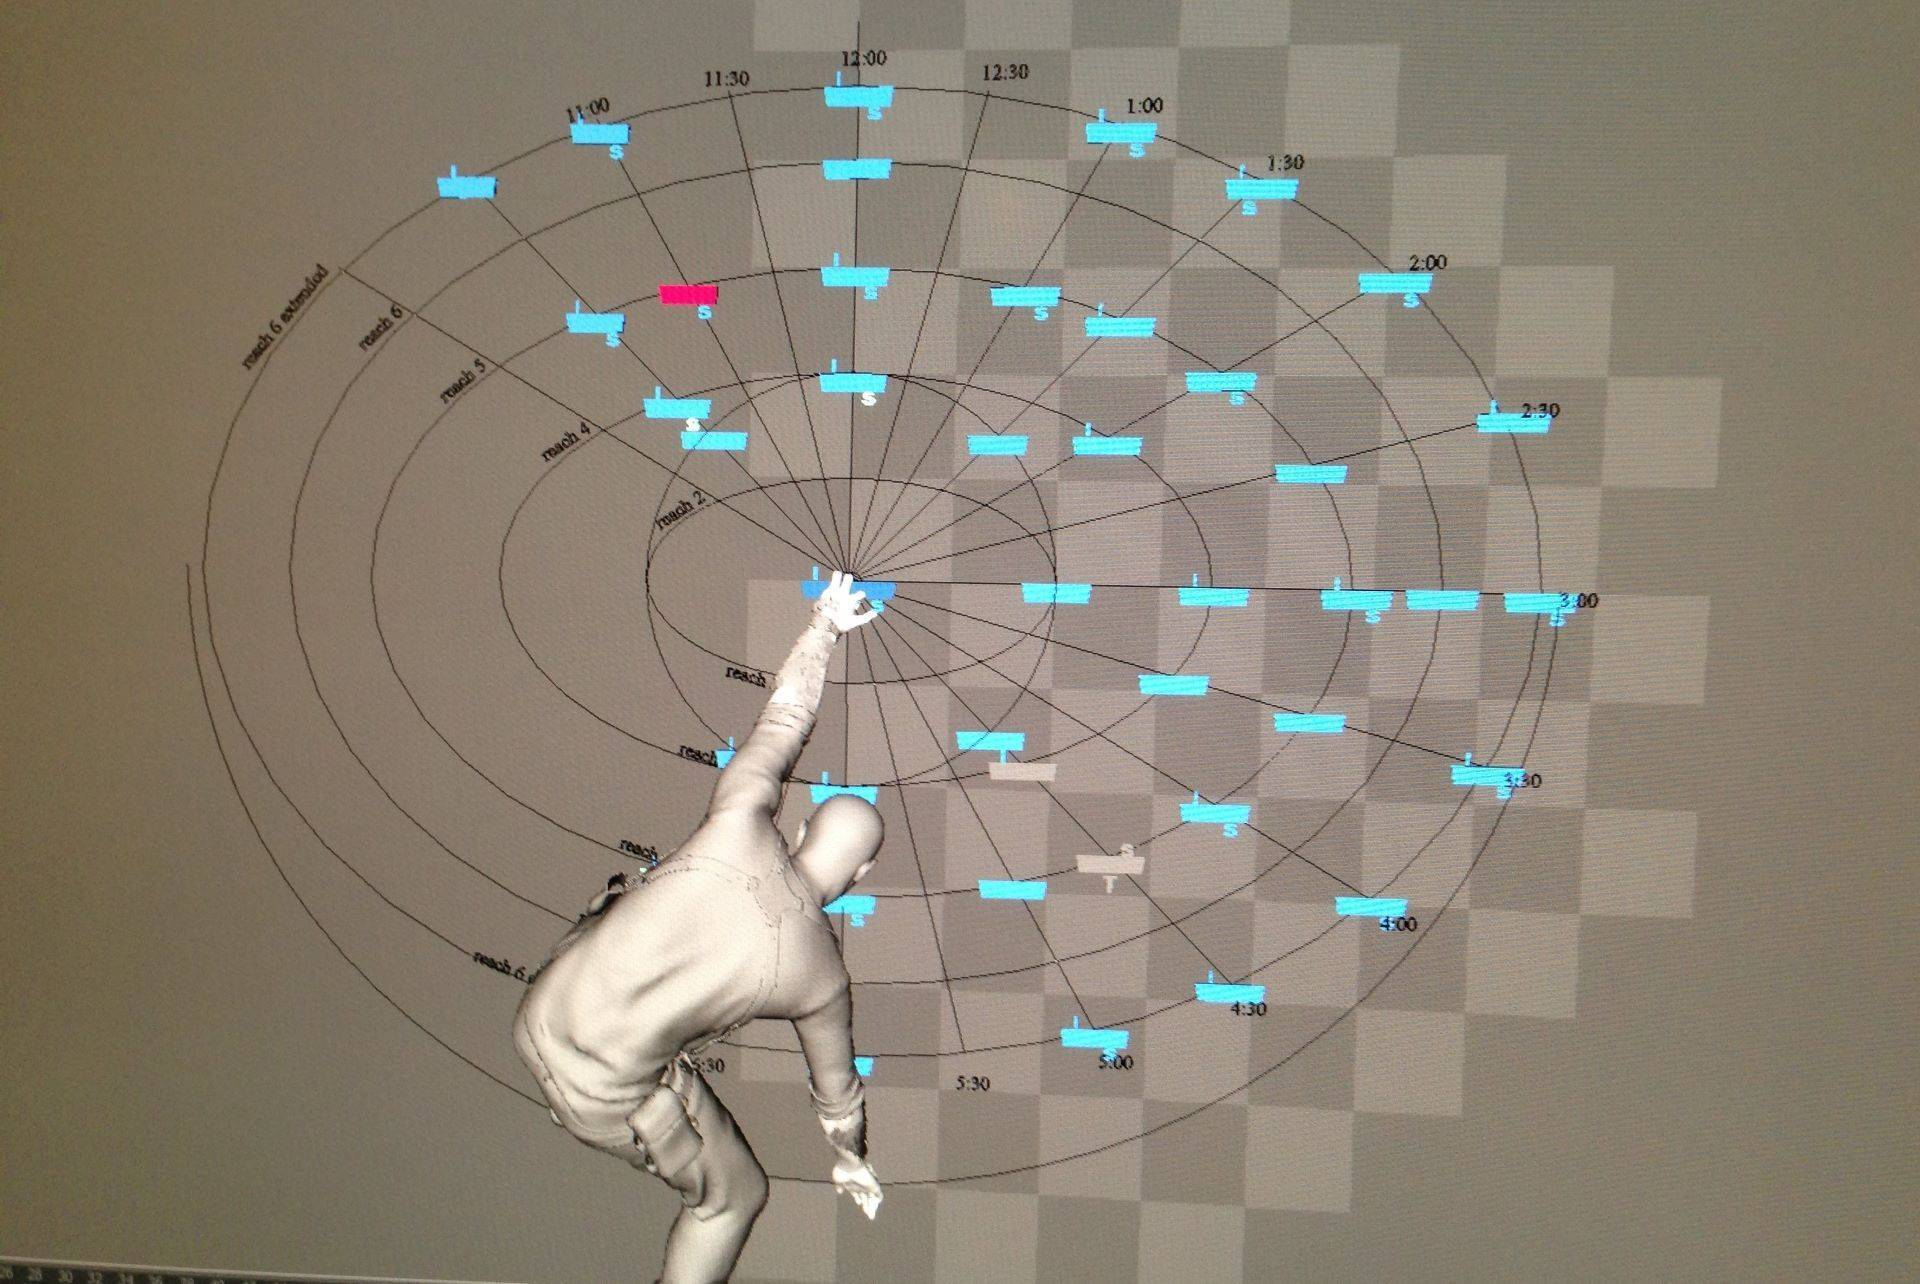
\includegraphics[scale=0.125]{climbing-reach-diagram.jpg}
\caption{Uncharted 4 (2016) uses an inverse kinematic solver to create dynamic climbing mechanics that react to the world around them based on player input.}
\end{figure}


\section{Technical Background}
At its most basic, an inverse kinematic (or IK) solver positions a system of joints such that the final joint, or end effector, is as close as possible to an input target position. In doing so, the chosen IK algorithm calculates the position and rotation of each joint from the anchored root to the final end effector. The majority of IK algorithms utilized in modern media are iterative. As such, in real time applications like game development a lightweight semi-realistic algorithm is preferable to a complex but highly precise implementation \cite{litReview}\cite{ZucconiIK}.

To this end, when choosing an IK algorithm for a character animator there are a few key factors to consider. The first is simply the speed of the algorithm. When using IK in games the algorithm will be run at best one time per frame (assuming an acceptable solution is found on the first iteration). An IK algorithm used for games needs to solve in under 16 ms at the absolute slowest. This assumes a game running at 60 frames per second and no other significant weight on the system. The second key factor is iterative efficiency. As previously stated, IK algorithms will solve sequential arrangements of joints until the target is within an acceptable tolerance range. The efficiency of an IK solver relies not only on how fast each iteration is but also on how many iterations are needed to solve the system \cite{litReview}\cite{baseFABRIK}. Fewer iterations leads to a faster solution which in turn means an efficient and reliable algorithm. The final factor in choosing an IK algorithm is realism. IK solvers used to animate game models need to create realistic poses in order to offer a true alternative to traditional keyframe animation. Meaning, the algorithm must move joints from one target position to another smoothly while also maintaining realistic joint angles and positions. Because of this, many fast and iteratively efficient algorithms are not suitable for game development purposes. 

There are countless IK algorithms, all with their own benefits and drawbacks within the aforementioned factors. The process of selecting an algorithm for use in a game engine starts by trimming down the set of available algorithms by considering what actions the character controller will need to perform. \textcite{spore} for example created a particle based IK system for the game Spore (2008) to project singular predefined animations like dancing and fighting onto the innumerable creatures that the player creates and modifies as part of the core gameplay loop. While particle IK systems can be fine tuned for just about any use case, the complexity of implementing this algorithm far outweighs the potential benefits when animating a static joint configuration. 

Another factor that makes it easy to trim several well researched algorithms from the search is the common use of complex matrix calculations. These can compound quickly in systems with higher degrees of freedom such as a multi-end effector system or long joint chains. This rules out the versatile Physics based Newtonian methods as well as Jacobian solvers that are popular in the field of Robotics for their accuracy and reliability \cite{newtonian}\cite{jacobianSingularity}. Despite being some of the most researched and reliable methods both of these families of algorithms utilize a number of matrix transformations and calculations to achieve their precision results, making them them unnecessary for a lightweight character animator \cite{litReview}.

Cyclic Coordinate Descent is a noteworthy algorithm that was a popular choice for game developers in the 2000s to animate characters and limbs. It is a heuristics based forward kinematic solver that rolls and unrolls a limb to iterate towards a solution by minimizing the distance between the end effector and target\cite{CCDBlog}. CCD converges quickly, is lightweight, and has been implemented to great effect in games like Shadow of the Colossus (2005) for both humanoid and creature animation systems \cite{ShadowofC}. CCD does have some drawbacks however. Firstly, it requires significant and expensive alteration to extend well from single joint chains to systems with multiple end effectors. Second, it can suffer from singularity issues making certian target positions unreachable. Finally, CCD can produce unrealistic poses due to the rolling and unrolling movements the algorithm uses to reach its target. For these reasons CCD is often blended with keyframe animations, extending the predefined motions to changing scenarios like idling on uneven ground or pointing a finger at moving targets \cite{baseFABRIK} \cite{CCDpaper}. Cyclic Coordinate Descent is a powerful IK solver but in recent years more flexible heuristic solvers have become more common.

FABRIK, or Forwards And Backwards Inverse Kinematics, is one of the most utilized IK solvers in the modern day. FABRIK solves joint systems by treating joint-bone relationships into points connected by vectors of constant length. This makes it simple to implement, computationally cheap, and suitable for most applications where the believability of poses is more important that the precision of the movement to get there \cite{FABRIKoptimized}. FABRIK converges quickly and creates believable poses that consider current joint positions to solve with minimal adjustments \cite{baseFABRIK}. Additionally it is easy to expand and constrain for complex models with multiple end effectors like a human skeleton \cite{extendFABRIK}. This makes it ideal for animation and has led to it being used in countless games from both large and small developers.


\section{Prior Work}

Forwards and Backwards Inverse Kinematics was first created by \textcite{baseFABRIK}. Aristidou's original study demonstrated FABRIK’s ability to produce natural looking poses for a variety of models. Additionally, the study posed a framework for constraining joints using a series of vector projections and transformations to restrict poses and create more realistic models \cite{extendFABRIK} \cite{quadruped}. Aristidou and Lasenby’s data shows that FABRIK vastly outperforms the speed and number of necessary iterations of CCD, Jacobian, DLS, and other popular solvers in both single and multiple end effector tests. 

\begin{figure}
\begin{subfigure}{.4\textwidth}
  \centering
    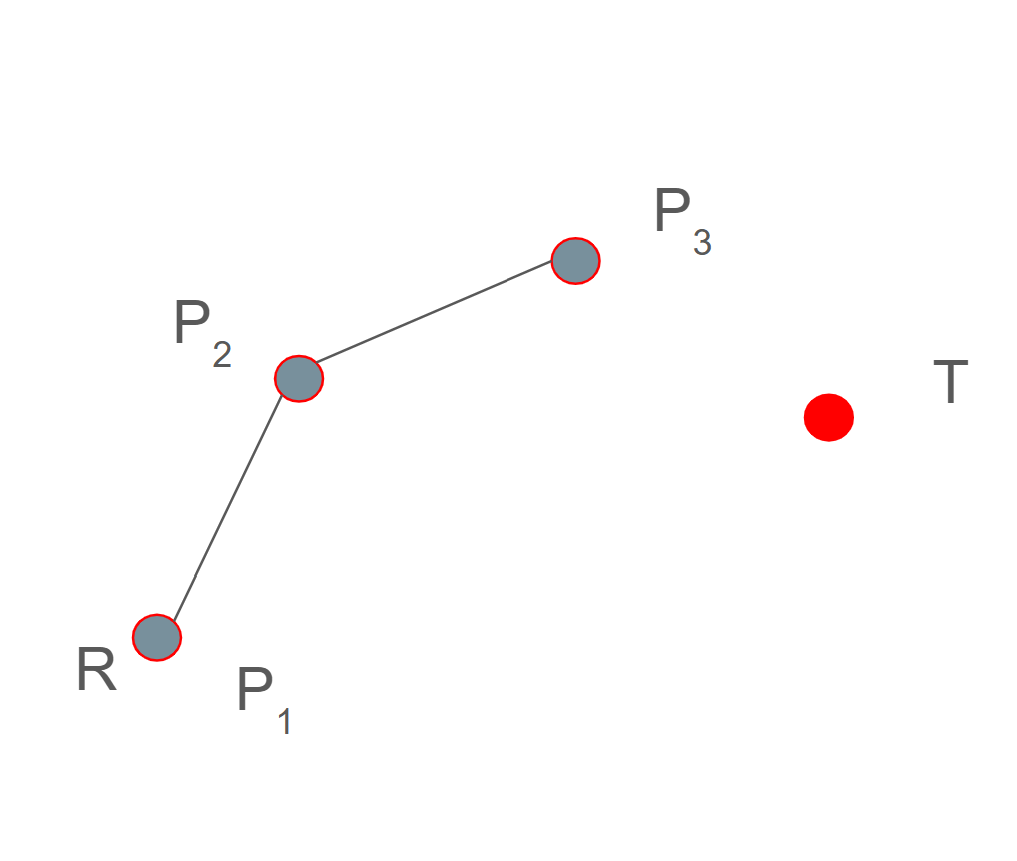
\includegraphics[scale=0.4]{start.png}  
    \caption{Initial state of the joint structure}
  \label{fig:sfig1}
\end{subfigure}
\begin{subfigure}{.4\textwidth}
  \centering
    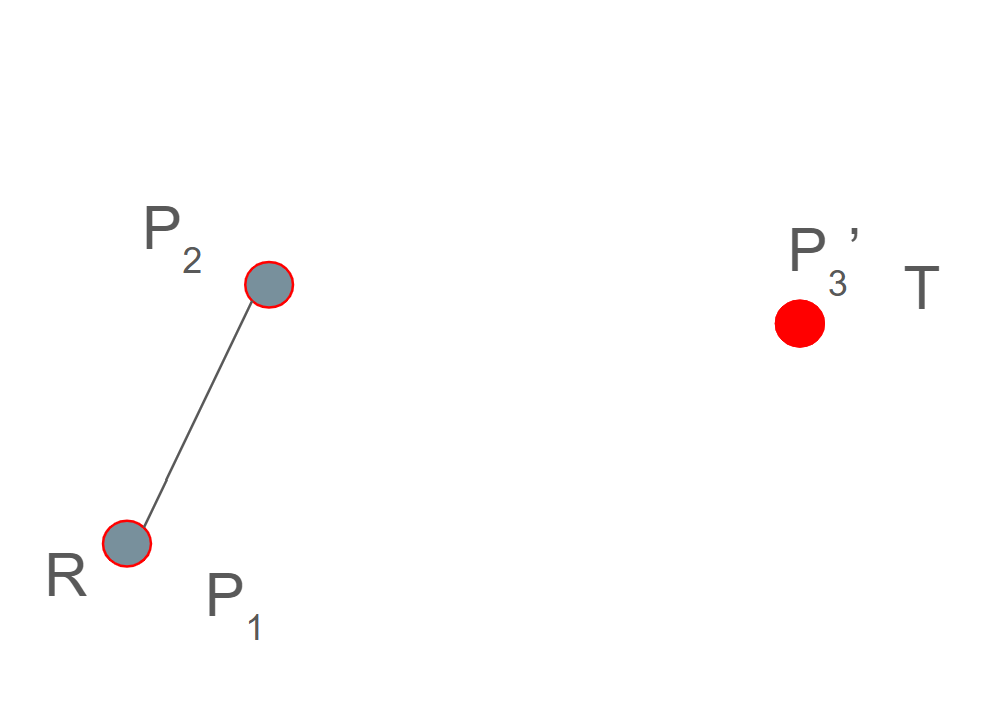
\includegraphics[scale=0.4]{step1real.png}  
    \caption{End effector is moved to the target position}
  \label{fig:sfig2}
\end{subfigure}
\begin{subfigure}{.4\textwidth}
  \centering
    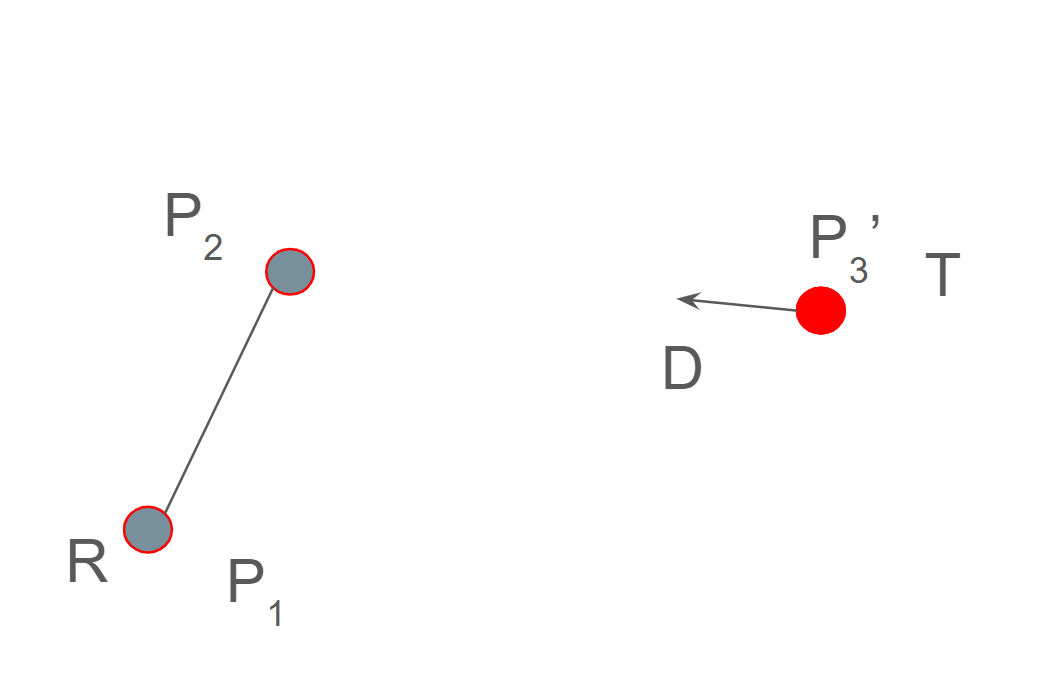
\includegraphics[scale=0.4]{step2.png}  
    \caption{direction vector $D$ is found from $P_i$ to $P_{i-1}$}
  \label{fig:sfig3}
\end{subfigure}
\begin{subfigure}{.4\textwidth}
  \centering
    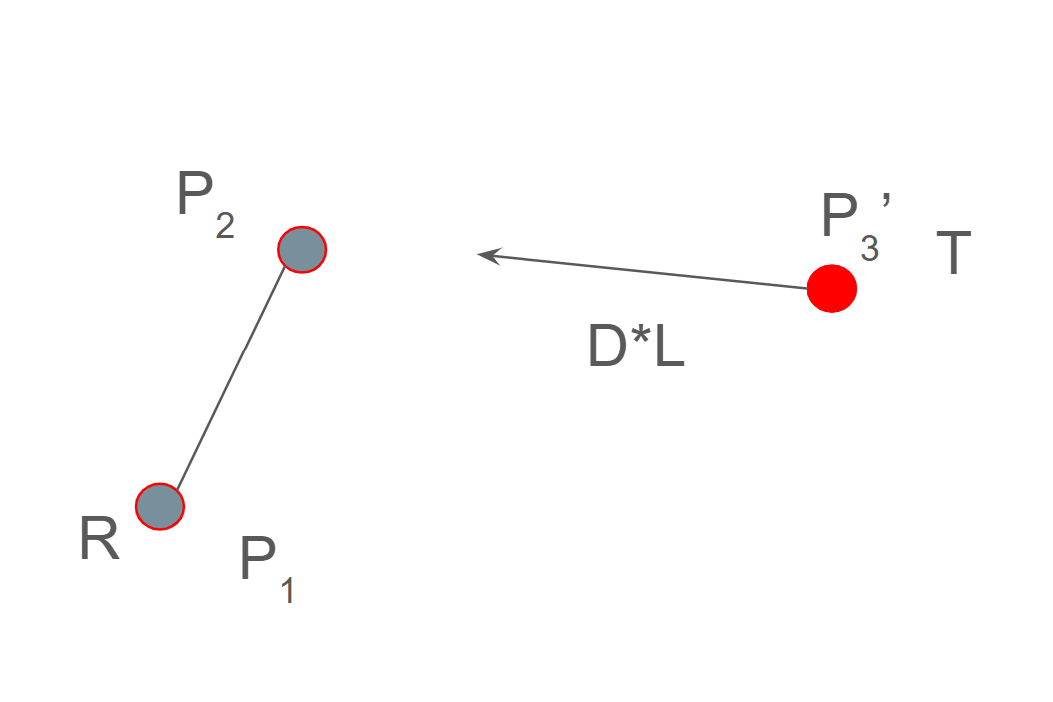
\includegraphics[scale=0.4]{step3.png}  
    \caption{D is multiplied by bone length $L$}
  \label{fig:sfig4}
\end{subfigure}
\begin{subfigure}{.4\textwidth}
  \centering
    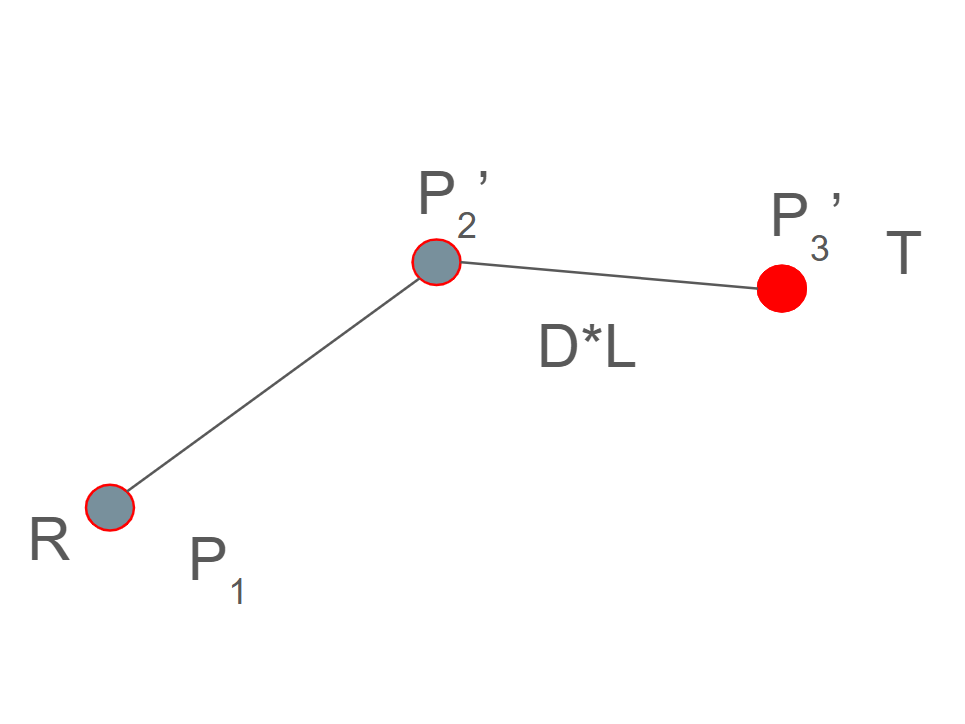
\includegraphics[scale=0.4]{step4.png}  
    \caption{$P_{i-1}$ moves to the end of the lengthened $D$ vector}
  \label{fig:sfig5}
\end{subfigure}
\caption{This diagram shows the first backward step of the FABRIK algorithm. This would be run for each joint before being reversed and run as the forward step.}
\label{fig:fig}
\end{figure}

FABRIK processes a limb as a series of joints $P_1...P_i$ where each joint stores its own position and rotation. Additionally, joints must remain at a fixed distance or bone length $L$. It should be noted that for more complex systems each joint may hold a different bone length represented by $L_1...L_{i-1}$; However, for the sake of simplicity a uniform $L$ value will be assumed. Finally, the root joint $P_1$ needs a root position, $R$, and the end effector $P_i$ needs a target position, $T$.

Given these inputs, FABRIK solves the inverse kinematics problem as a two step process. Firstly, in the backward reaching step the position of the end effector $P_i$ is set equal to the target position $T$ creating the start of the updated system at $P_i’$. The difference in positions between $P_i’$ and the next joint in the chain, $P_{i-1}$ forms a vector pointing backwards towards $P_{i-1}$. Normalizing this vector and multiplying it by the joint length $L_{i-1}$ creates a position vector $P_{i-1}’$  that preserves the constant bone length. This process is then repeated until the root joint $P_1$ is updated and a full backward pass is completed. 

The forward reaching step follows the same algorithm but in reverse. $P_1$ is placed directly on the root position $R$, a vector pointing towards $P_2$ is calculated, This vector is scaled to size $L_1$ to find $P_2’$. Again, the process is repeated until the end of the chain is reached which completes a single iteration of the base FABRIK algorithm. Following this reach and pull strategy creates realistic poses with a small number of iterations \cite{baseFABRIK}\cite{extendFABRIK}\cite{FABRIKoptimized}. Figure 2 illustrates a backward step of the FABRIK algorithm in 2D. 


\begin{figure}[h]
\centering
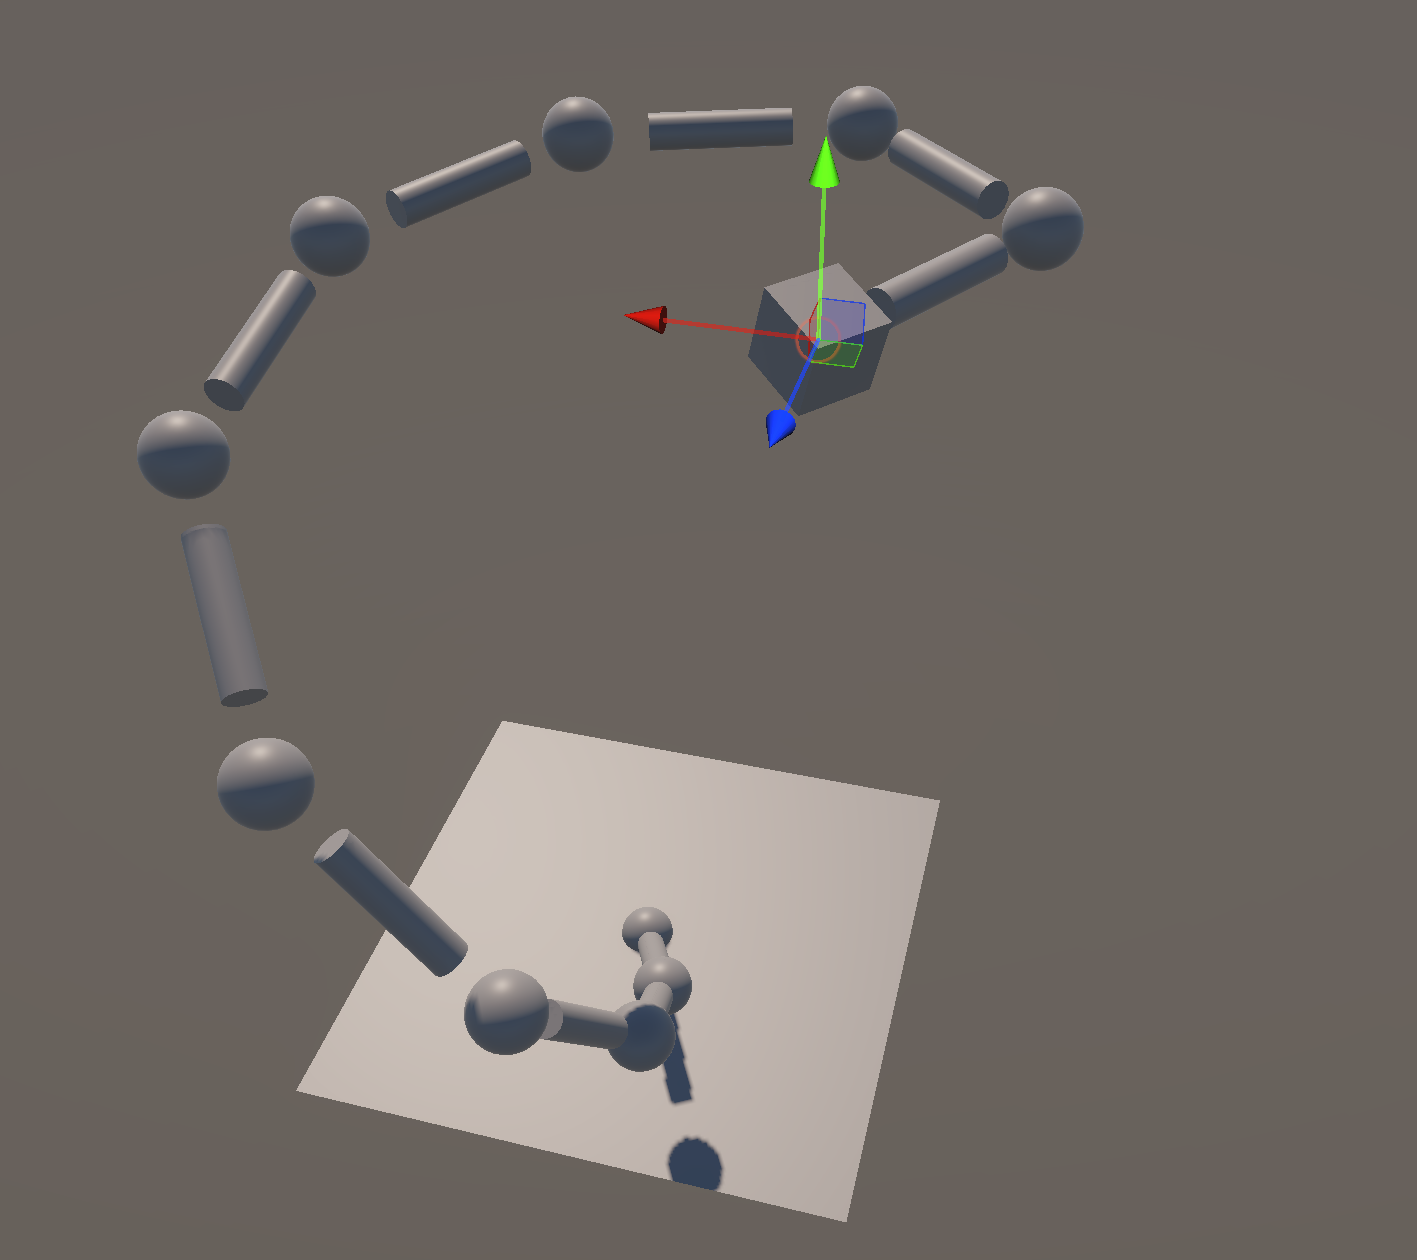
\includegraphics[scale=0.45]{FABRIK3D2.png}
\caption{A single end-effector model showcasing organic movement and poses using the unconstrained FABRIK algorithm. Created in Unity 3D}
\end{figure}


\textcite{extendFABRIK}, Aristidou and Lasenby’s supplementary research on constrained FABRIK models, explores performance in edge cases as well as the feasibility of implementing realistic biological joints. They were able to implement basic pivot, ball and socket, and hinge joints using their unmodified constraint model. However, condyloid, saddle, and plane joints required alterations to the algorithm to allow inter-joint distances to fluctuate with movement. This research makes their vector based constraint model a desirable option compared to other IK constraint schemes like quaternion rotation constraints or Polar coordinate restrictions \cite{CCDpaper}\cite{CCDBlog}. It’s worth noting that the infeasible joint types that require alterations can be largely ignored in a game development environment as a convincing product can be made with only pivot, ball and socket, and hinge joints when constrained properly. 


\section{Model Design Methods}

\subsection{Multi-End Effector Model Structure}


 The focus of this research is a model built in the Unity 3D game engine. Unity allows each joint to exist as its own child object positioned by a single parent body that runs the FABRIK solving script. For ease in up-scaling and management, each joint object inherits a base FABRIK joint class that stores unique information like bone length, parent joint object references, and important calculation functions that rely on local data and transforms. This is helpful when adding joint types and constraints later on. All joints are referenced and controlled by the central body script that organizes and solves the chain using the modified FABRIK algorithm. Figure 3 shows this basic form of 3D FABRIK running on a single end effector chain in Unity. 

Scaling a single end effector chain up to a complex skeletal model is fairly simple. Complex models rely on the fact that FABRIK chains always return to their root at the end of an iteration. Solving several chains with a shared root joint creates a connected model with multiple end effectors. Then, by connecting two of these systems we have effectively created an upper body and lower body with a spine between them. It is important to note that the upper body’s root, hereby known as the upper chest joint, is functionally the end effector of the spine but its position remains the root of the arms and neck while the lower body’s hip joint will become the root joint for the entire body. This means that even if the upper chest target is unreachable, the arms and neck will remain attached to the joint’s final solved position keeping the model connected and cohesive \cite{baseFABRIK}\cite{FABRIKoptimized}\cite{animalsIK}. 

With a final structure in place there are two more structural considerations. First is the order in which joints are solved. Joints can’t be solved at the same time because the spine’s position influences the roots of all other limbs. As such, the spine is solved first, followed by the legs, arms, and finally the neck. Second, rotation is a tricky problem in FABRIK especially with multiple constrained joints influencing on one another. The rotation of a joint earlier in the limb will come to affect those further down the chain. As an example, a shoulder’s rotation decides the axis on which the hinged elbow will be constrained. Consequently, the upper chest and hip joints have a significant impact on the orientation of the entire skeletal system and should be positioned independently of other joints. These joints are called subbases and they are hard-coded to always face “forward” or (0,0,1) in the model's local space. Forward  may be defined differently for specific use cases but this model remains stationary for testing so forward can be reasonably assumed to point in one direction \cite{extendFABRIK}.

\begin{figure}[h]
\centering
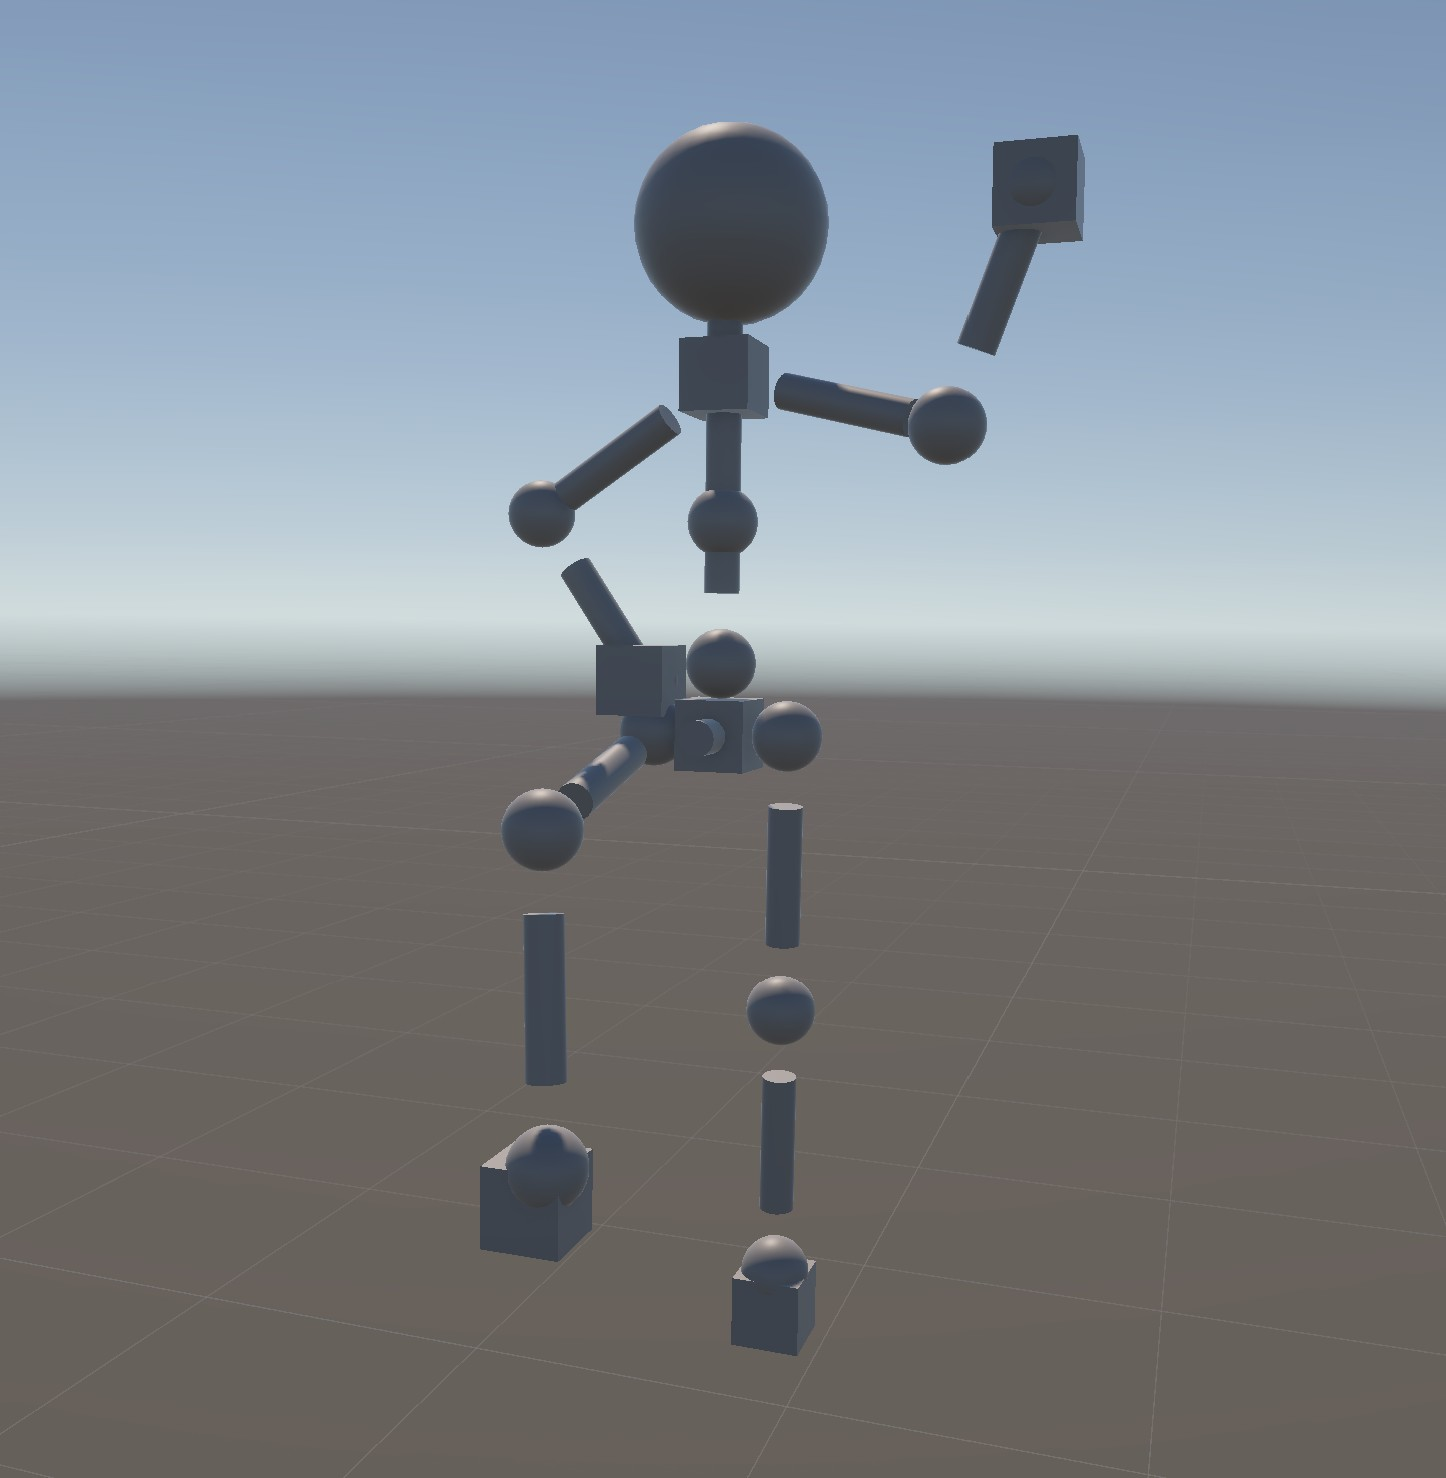
\includegraphics[scale=0.5]{Poster2.jpg}
\caption{A positionally constrained skeletal model in a solved position. Created in Unity 3D}
\end{figure}

With the skeletal object assembled, each joint must now be constrained to mimic human motion. These constraints fall into 3 categories: hard constraints on where joints can and cannot move, soft constraints which influence the solve process to achieve more probable postures, and joint resets which help the model transition in and out of extreme solve positions. Hard constraints made up the majority of the first section of this study while the later two constraints formed the second section. As such the explanation of the constraint types will be split up and discussed in the order they were implemented.

\subsubsection{Hard Constraints}

Hard constraints limit joint movement in line with the physical limitations of the human body. In this case, these constraints are purely positional and govern the boundaries of each joint’s allowed movement. Constraining positions in 3D is normally quite complicated and expensive, utilizing either Euler angles, which suffer from gimbal lock, or Quaternion transformations that become difficult to control when ranges of motion extend beyond a uniform spherical sector. In \textcite{baseFABRIK} the constraint framework relies on a series of vector projections to convert the 3D problem to 2D. This method can be applied to this study with some minor adjustments in order to create ball and socket, pivot, and hinge joints with semi-realistic ranges of movement. 

Regardless of the type of joint, the process of constraining its position utilizes the same base algorithm. All constraints take place on the forward pass where the model builds from the root node forward toward the end effector. As such, given the current joint being solved $P_i$, any joint $P_n$ where $n < i$ has already been constrained and solved. To constrain any unique joint in the solve sequence $P_i$ you must first apply the basic forward pass to find $P_i’$. Then both $P_{i-1}$ and $P_i’$ are projected onto a 2D plane that is orthogonal to the parent joint’s local X, Y or Z axis (the chosen axis depends on the type of joint being constrained. Ex. Upper leg joints are constrained on the local Y axis). This results in a 2D parent position $L$ and an ideal target position $O$. Then by subtracting $L$ from both points we translate such that $L$ is located at the origin of the 2D space. It is at this point that different joint types follow a different process.

Ball and socket are the most complex as they allow each quadrant of the 2D plane to be constrained individually allowing for a range of unique joints. Constraints in this 2D space are defined by 4 sets of intercepts each of which forms a line across a quadrant of the plane. For the sake of this example let’s assume a joint constrained on the local Z axis. For a joint with a square range of motion these could be defined as (1,1), (-1,1), (-1,-1), (1,-1). A joint like this is visualized in Figure 5. Any $O$ that sits between the quadrant's constraint line and $L$ is within the allowed range of motion while any $O$ outside of the quadrant line needs to be constrained. Should an $O$ value need to be constrained, the constrained $O’$ value for a set of points is found at the intercept of the quadrant constraint line and $L \rightarrow O$. Once $O’$ is found in the X and Y, its Z position must be located at one of exactly 2 points to conserve the joint length. One of these points must be positive and the other negative. 


\begin{figure}[h]
\centering
\boxed{
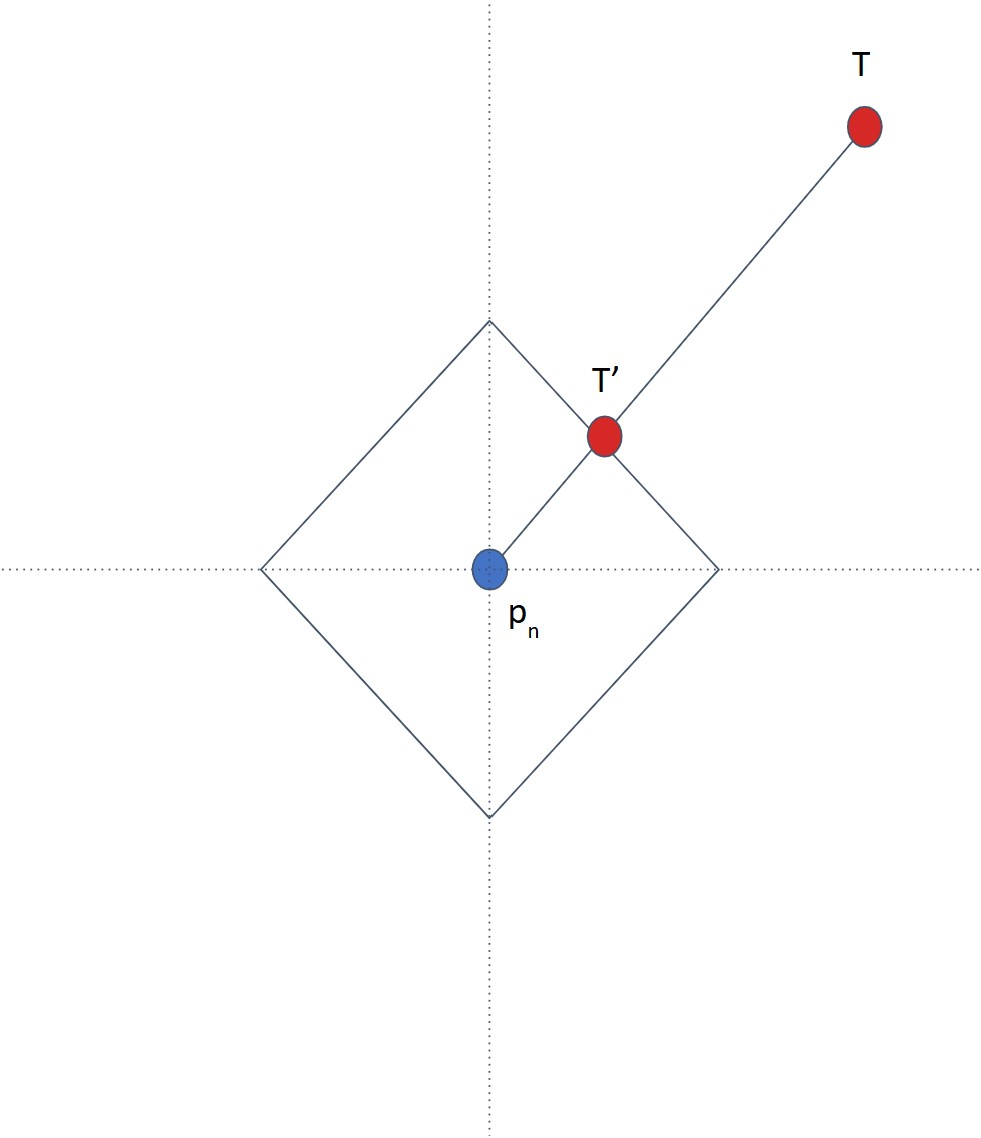
\includegraphics[scale=0.5]{constraint.jpg}
}
\caption{A ball and socket joint at position $P_n$ constraining the target position $T$ of a child joint using a square set of constraints}
\end{figure}

In some cases it is easier to force either the positive or negative Z result to keep the joint either strictly positive or negative Z. This is the case for shoulder joints as the vast majority of their movement range is in either the positive or negative side of the body. However, upper leg joints, which are constrained on the Y-Axis, need to allow both positive and negative Y values in order to move realistically. To allow this, 2 groups of constraint lines are defined. One of which is used when $P_i$’s  Y-Position is greater than $P_{i-1}$’s and the other of which is used when it is less. One of these constraint sets is inclusive such that $P_i'$ will be forced inside the constraint boundaries and the other is exclusive meaning $P_i'$ will be kept outside of the constraint boundaries. Pairing this with unique intercept values that extend beyond the joint length creates a hole in the constraint and allows passage from the negative Y hemisphere to the positive Y hemisphere. This process builds a 3D constraint boundary using only 2D line intercepts just like before, allowing the method to extend to joints with complex constraints. The final Y position can be solved to the result with the same sign as $P_i’$’s original Y-Position.

Hinge and pivot joints are much simpler. A pivot joint doesn’t allow movement, only rotation. Meaning that replacing the $O$ position with $L$ constrains the joint. Similarly, the process of projecting on a particular axis already creates a hinge joint for that axis. However, hinges don’t have unlimited movement on the axis. By measuring the angle $\theta$ between (1,0) and $O$ and setting maximum and minimum angles a valid $O'$ position is any point where $\theta$ falls between the maximum and minimum. If $\theta$ is too large or too small then $O’$ is a vector nearest limit angle with length $L$. For arms and legs this maximum angle can be easily defined as the parent joint’s forward vector projected into the 2D space. The minimum can then be reasonably assumed 180 degrees less than the maximum \cite{baseFABRIK}\cite{CGjointStructure}.

With $O’$ found, $L$ is then added to $O’$ to undo the original translation and $O’$ replaces $P_i$.This process then continues down the joint to the end effector. It is also worth noting that this process is much easier to perform on a standard XY 2D plane. This can be achieved by measuring the rotational offset from the constraint axis to $P_{i-1}$'s rotation as a quaternion and inverting it to get $Q$. Multiplying $Q$ and $O$ removes $P_i$'s rotation allowing the constraint intersections to be measured in the standard XY coordinate system. After constraining, re-inverting the quaternion value to get $Q^{-1}$ and multiplying with $0’$ re-applies $P_{i-1}$'s rotation. This simplifies calculations but still allows joints to be constrained within the scope of their parents \cite{swingTwist}\cite{Quaternions}.

\subsubsection{Soft Constraints}


Soft constraints don’t explicitly limit the movement of the model but they do make adjustments to the model’s posture to make it more human-like. The main way they achieve this is by influencing joint rotation. A good way to highlight the need for rotational constraints is by thinking of a shoulder that can rotate 360 degrees in its socket. While the attached elbow may be a hinge joint in theory, it regains its third degree of freedom through the rotation of the shoulder. This leads to odd solutions and postures when running the FABRIK algorithm for hundreds of iterations. It's worth re-emphasizing that parent joints influence their children, so the rotation of the shoulders and upper legs hold most of the influence over the solved positions of the arms and legs. 

Rotations in Unity are quaternion values, but quaternions can be decomposed into swing and twist values. The swing influences where the object is pointing, but the twist decides which way is up. When building quaternions you can use 2 vectors to represent the swing and twist. These are called the forward and up vectors. The forward vector of any joint in this model simply points at the next joint in the chain (i.e. The shoulder points toward the elbow and the elbow points toward the hand). However, the up vector is where soft constraints steer the posture of the model.

The biggest problem with constraining rotation in the upper leg and shoulder is that they are the first joints in their chain and their rotation must be set as the next joint is solved. This means that the only information available is the joint’s forward vector $F$ and the target position $T$. These are enough to make a pretty good guess at how a real leg would be oriented simply because an intermediate hinge joint needs to have its constraint axis aligned with the target in order to be able to reach it. This means that the up vector $U$ for the root joint at $P_1$ should be orthogonal to the normal of a plane defined by corners $P_1$ and $T$. Finding the cross product of $F$ and $P_1  \rightarrow T$ gives the normal for that plane $N$. So, $N \times F$ returns a possible up vector for the joint that will work with the required $F$ value.

In reality this must be constrained slightly more in order to fit realistic ranges of movement but the math above gets most of the way there. For leg joints this means keeping the local Z value facing the positive direction while the local Y is negative and vice versa when Y is positive. Similarly, shoulders are mirrored so the up vector’s X value should always be positive for the right shoulder and negative for the left shoulder. With the shoulders and upper leg rotations finalized the knee and elbow joints can adopt their parent's up vectors to stay oriented on the same plane as their targets. 

\begin{figure}[h]
\centering
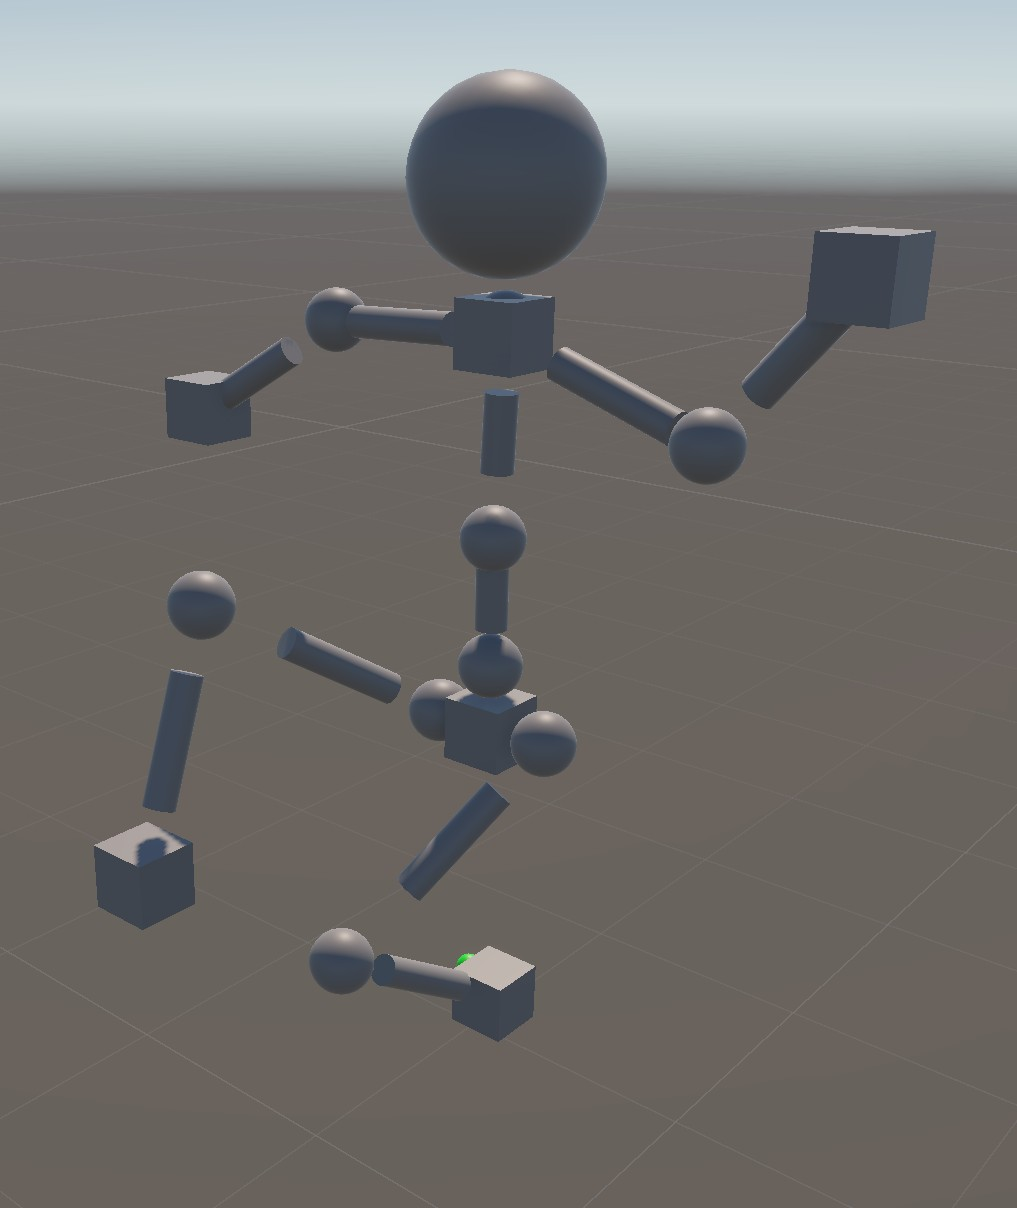
\includegraphics[scale=0.45]{pose1.jpg}
\caption{A fully constrained FABRIK model solving a complex pose}
\end{figure}

\subsubsection{Model Resets}

Constraints help FABRIK solve a skeleton in a more realistic way by creating barriers to prevent unlikely and problematic solutions. Yet, it is also possible for the constraint barriers obstruct the path from one solved position to another. This becomes troublesome due to FABRIK’s iterative nature. Single errors can compound and force the model into problematic configurations that continue to interfere with solutions. It is possible to prevent these compounding issues by forcing the model into a neutral state periodically before solving. 

After experimenting with different reset positions, the configuration shown in Figure 7 proved to be the best for creating consistent solutions that remain smooth even when the model is reset every frame. The configuration is mostly just a T-Pose to allow the spine to straighten and arms to bend from an extended state but the legs proved to be problematic when starting from a fully extended pose. The legs in this model are the most heavily constrained joint system. This paired with their specialized ball and socket joint with a wider range of motion makes it difficult to properly position the knee joints, especially when they should be above the hip. Because of this it was more beneficial for the leg reset position to be detached from the body and raised above their range of motion. This allows the model to solve from the top down, which keeps the knees in a raised state by default only to be corrected if necessary. 

\begin{figure}[h]
\centering
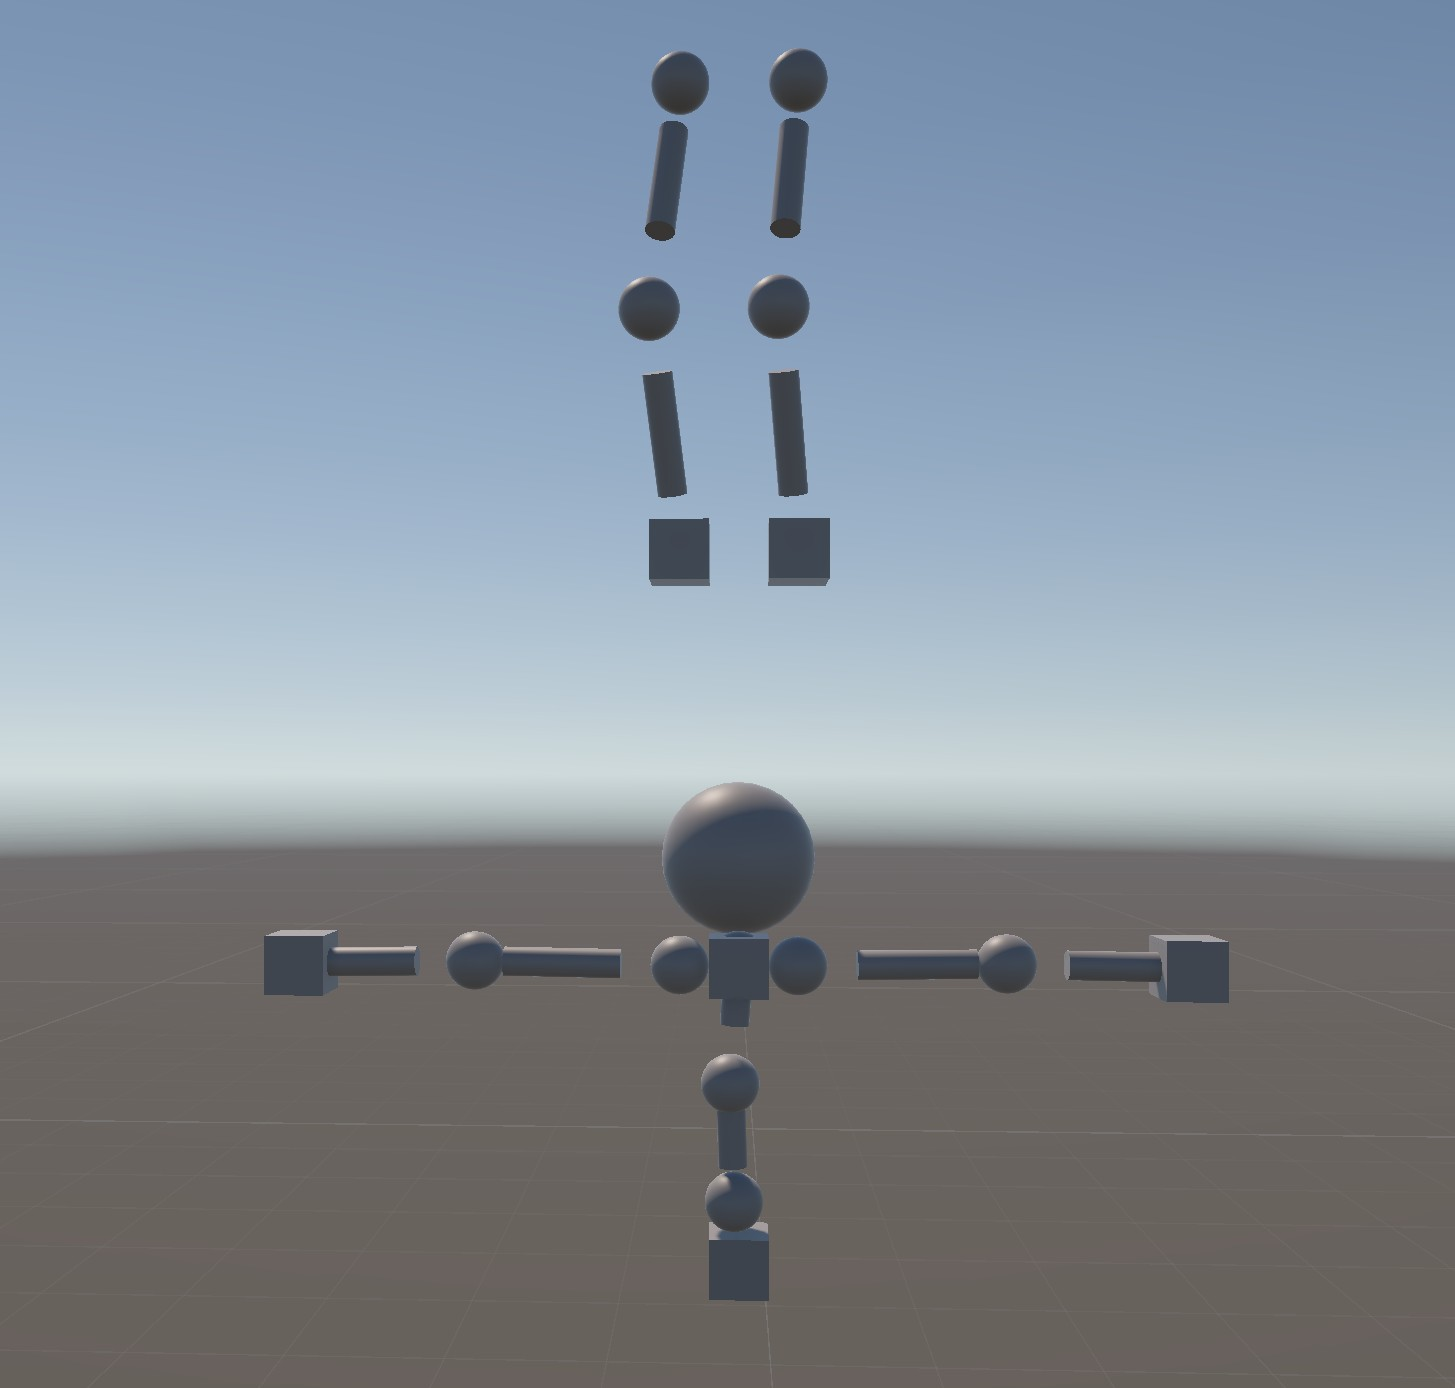
\includegraphics[scale=0.45]{reset-pose.jpg}
\caption{The reset positions used in this model. }
\end{figure}


 \section{Experiments}

To measure the versatility and accuracy of the FABRIK skeletal model it was tested against motion capture data gathered using Sony Mocopi sensors. Mocopi's customization capabilities allowed test data to be recorded using sensors placed on the body to mimic the locations of the targets that the FABRIK model uses to update joints. 2 animation segments were recorded, uploaded to Unity, and applied to a standard humanoid rig. The FABRIK targets were then set to follow the wrists, ankles, head, chest, and hips of the motion capture armature such that the FABRIK model would mimic the recorded movements. Then, by measuring the offsets between the motion capture armature and each corresponding FABRIK joint, different constraint configurations could be tested against one another to see which was able to mimic human movement the best. A perfectly tuned model would be able to follow closely from frame to frame and would see an average joint offset near the set tolerance range. For these experiments the tolorance range was set to 0.1 Unity meters and all models were given a maximum of 10 iterations per frame before offsets were measured \cite{FABRIKMocap}\cite{benchmarkGit}. 

 \begin{figure}[h]
\centering
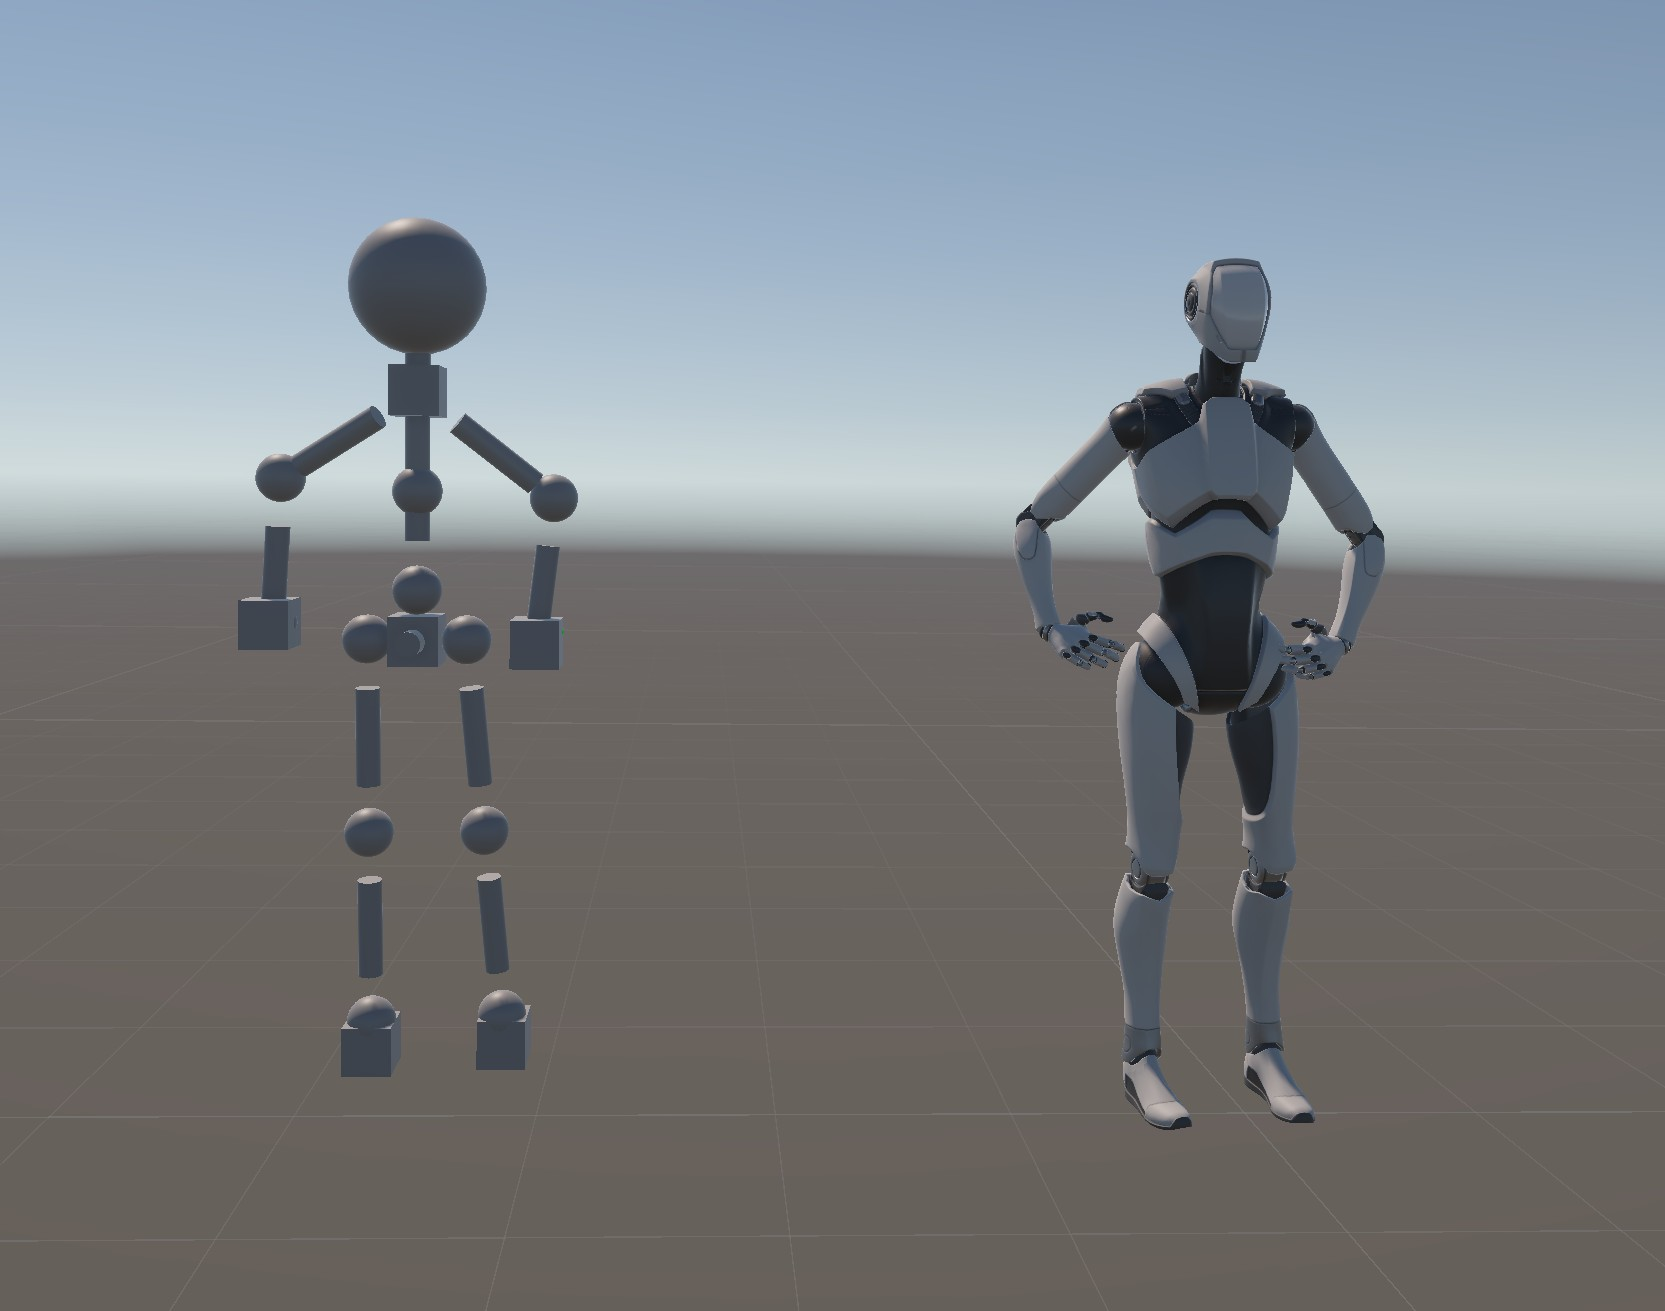
\includegraphics[scale=0.45]{Poster1.jpg}
\caption{FABRIK skeletal model (left) matching the pose of a motion capture animated model (right).}
\end{figure}

The first motion capture recording exclusively used sensors located at body positions with one to one FABRIK targets or roots. The second recording was gathered with extra sensors at intermediate joints on each limb. In this case extra sensors were placed at the upper arms and upper legs to allow better tracking of knee and elbow joints. Using this data the same tracking test was run but with increased confidence in the accuracy of the intermediate joints of the motion capture data. While tracking end effector offsets measures how well the FABRIK model can reach its target, measuring intermediate joint offsets gives a better look at how well the model can mimic human poses and movements in their entirety. 

Before discussing the results of these tests it is important to note that the skeletal armature animated with motion capture is not equivalent to the skeleton built by the FABRIK model. The motion capture armature has extra joints throughout the spine, neck, and chest which makes it difficult to precisely measure and mimic the joint lengths of the model when constructing the FABRIK skeleton. 


 \section{Results}

\begin{table*}[]
\centering
\caption{Test 1 Results}
\resizebox{\textwidth}{!}{
\begin{tabular}{l|lllll|lll}
                       & Hands   & Elbows  & Feet    & Knees   & Shoulder & EE Mean & Interm. Mean & Combined Mean  \\ \hline
Unconstrained Model                          & 0.07349 & 0.71005 & 0.20850 & 0.29744 & 0.00001  & 0.14222           & 0.50375           & 0.30290                \\
Position Constraints Only                    & 0.54920 & 0.68589 & 0.90474 & 0.28377 & 0.00001  & 0.58157           & 0.48483           & 0.53858               \\
Rotation Constraints Only                    & 0.06164 & 0.72857 & 0.20928 & 0.29382 & 0.00001  & 0.13771           & 0.51120           & 0.30370                \\
Position and Rotation Constraints            & 0.08248 & 0.66587 & 0.77685 & 0.30588 & 0.00001  & 0.39438           & 0.48588           & 0.43505                \\
Position With Reset                          & 1.06397 & 0.30334 & 2.77845 & 0.25258 & 0.00001  &  0.97741            & 0.27796           & 0.97741                \\
Rotation With Reset                          & 0.12403 & 0.2308  & 0.23113 & 0.24082 & 0.00001  & 0.17424           & 0.23582           & \textbf{0.20161}                \\
Fully Constrained & 0.12696 & 0.23035 & 0.45743 & 0.23533 & 0.00001  & 0.28361           & 0.23284           & \textbf{0.26105}               
\end{tabular}
}
\end{table*}

\begin{table*}[]
\caption{Test 2 Results}
\resizebox{\textwidth}{!}{
\begin{tabular}{l|lllll|lll}
                       & Hands   & Elbows  & Feet    & Knees   & Shoulder & EE Mean & Interm. Mean & Combined Mean \\ \hline
Unconstrained Model                          & 0.11947 & 0.69084 & 0.20292 & 0.31910 & 0.00001  & 0.15943           & 0.50497           & 0.31301                \\
Position Constraints Only                    & 0.65640 & 1.17266 & 0.37993 & 1.32274 & 0.00001  & 0.86641           & 1.24770           & 0.86641                \\
Rotation Constraints Only                    & 0.10719 & 0.70104 & 0.19866 & 0.31522 & 0.00001  & 0.31069           &  0.50813           & 0.31069                \\
Position and Rotation Constraints            & 0.14402 & 0.60313 & 1.03195 & 0.29467 & 0.00001  & 0.52323           & 0.44890           & 0.49019               \\
Position With Reset                          & 1.50141 & 0.48408 & 1.85327 & 0.27703 & 0.00001  & 1.34187           &  0.38056           & 0.91462                \\
Rotation With Reset                          & 0.16006 & 0.43944 & 0.43944 & 0.26781 & 0.00001  & 0.25916           & 0.35363           &\textbf{0.25916}                \\
Fully Constrained  & 0.20684 & 0.48673 & 0.35553 & 0.28683 & 0.00001  & 0.28249           & 0.38678           & \textbf{0.32884}              
\end{tabular}
}
\begin{description}
    \item[Tables 1 and 2:] Results from test 1 and 2 comparing the FABRIK model's solved position against the ground truth motion capture data. The right side of the table shows end effector mean, intermediate joint mean, and total mean distance between the model solution and motion capture position. The near-zero shoulder values here are a result of the solve order. The neck solves last, using the shoulder target as a root so the shoulder joint is always perfectly solved.
\end{description}
\end{table*}

Tables 1 and 2 show the results of the animation offset experiment on every permutation of constraints. Note that table 1 shows the test without extra sensors in the data gathering process so intermediate offsets show the difference between this study’s FABRIK model and a commercial inverse kinematics product.

The base FABRIK model provides a solid base case for the model’s ability to mimic human movement. As expected, an unconstrained model is able to come very close to all end effector positions, as it faces no barriers there, but performs significantly worse for the intermediate joints placed purely by the movement of the target. Equally as expected is the dip in performance from the position-only constraint model. As previously mentioned, positional constraints serve as a barrier for the model’s movement without informing the movements themselves. So, while they prevent impossible poses, positional constraints alone are not able to create realistic movements through FABRIK. Slightly more surprising is the dip in performance when adding resets to the positional model. Usually this helps circumvent the pitfalls that positional constraints create but they also make the model deterministic in that it solves from the same starting position every frame. In this case it seems that uninterrupted iteration is more helpful for a purely positional model. 

Rotation constraints on their own don’t have much impact on the model. Both the resulting offsets and the solved positions throughout the tests closely mirror the unconstrained model. Without positional constraints on the hinged knees and elbows, rotation has very little impact on FABRIK. However, when positional constraints are present the addition of rotation constraints always increases performance. The combination of all three constraint methods produces results that show both accurate tracking of targets and acceptable posture. These results show FABRIK’s versatility and how it could be able to adapt to many use cases.

The best combination of constraints for matching motion capture data completely excludes positional constraints. The rotation constrained model with model resets was able to follow both animations with an extremely small margin of error across all joints. Initially this result suggests that positional constraints are unnecessary and only hinder performance; however, motion capture data is already constrained to human joint limits because it is gathered through real human movement. What these results do show is that the existing constraints are too restrictive to mimic this set of movements. They also show that solving from a beneficial starting position is incredibly important for the FABRIK algorithm. Model resets remove one of the key qualities of FABRIK in favor of a consistently beneficial starting pose. These results show that this technique improves results for any model that is already approaching the unconstrained baseline.



\section{Discussion}

\subsection{Ethical Considerations}

The ethical considerations of inverse kinematics are as varied as the applications. Procedural animation on its own is not a risk to security, privacy, or personal freedoms but some of its applications can raise concerns in these areas. Animated media is like all other forms of media in that it must be created and maintained responsibly. Providing easily accessible animation tools to developers does create a risk of irresponsible use; however, when considering the wide array of free animation applications available to the average consumer and the limited scope of this research it is clear that this FABRIK skeleton model does not pose any additional ethical risks.

\subsection{Code Overview and Replication Instructions}

The FABRIK skeletal model as well as the building blocks used in its creation are built in Unity 6.0. As such, downloading the game engine and opening the source files as a new project will automatically create all of the dependencies needed to recreate the results from this paper. All of the scripts, object prefabs, and other files utilized in the creation of this process are stored in the Assets folder of the Unity project files. The source code is available at: github.com/PlutoPotatoes/FABRIK-Procedural-Armature.

Building upon these results for further research or creating a customized skeletal model may take a more in-depth understanding of how this model interfaces Unity's object oriented engine. The experimental model that this paper focuses on uses the FABRIKSolver script to organize and animate the skeleton. Skeletons that use this script or any derivative scripts must start with a empty parent 'body' object. Joint chains are then added as children of the body object such that they use the empty parent as their base world position. This lets the whole skeleton be moved as a single body which is essential if utilizing any form of character movement script. It is also important that the joints are not made children of one another. While this is a common technique for some animation rigs, this solver manipulates all joints in world space independently of their parent objects. Parenting the joints to one another will cause the movement of one joint to move all its children in the same manner. FABRIK builds each limb one joint at a time, so moving unsolved joints through parenting leads to inaccurate solutions. 

The FABRIKSolver script's serialized field variables allow it to store references to each joint's game object in order to manipulate their transforms at runtime. These references are organized into arrays for each limb so each array can be iterated during a forwards and backwards step to solve a single limb at a time. The solving process then runs the FABRIK algorithm on each of these arrays in a set order until a solved position is reached. 

Each joint game object has a FABRIK joint script that holds unique data each joint's bone length, constraint ranges, constraint axis, and a 'sidedness' variable. While most of these fields are self explanatory, sidedness is a bit more complicated. When a constrained joint is projected into 2D and solved it leaves 2 possible values for the 3rd Projected dimension that preserve the joints constant length. Because the constraint process translates the joint in question to the origin of the 2D plane we are also able to assume it is at the origin of the 3rd dimension's axis. As such, one of these values will always be positive and one will always be negative (excluding a zero value). Sidedness collapses this choice and picks either the positive or negative side of the 3rd dimension. This is eliminates positional snapping between the two possibilities and allows mirrored joints like shoulders to be reused on the other side of the body. Constrained joints inherit from a base joint class and override the empty constraint function with their specific algorithm. This structure allows each joint to be edited at runtime allowing the skeleton to be fine tuned with ease. 

All of the scripts that make up this project are built to be flexible building blocks that can be utilized to create any kind of skeleton. By adapting the FABRIKSolver script all joint, constraint, and utility scripts can be recycled to form the animation foundation for a wide variety of projects. 


\subsection{Conclusion}

Inverse kinematic solvers are utilized in a number of ways across different fields, each of which require a different level of precision and realism. FABRIK is lightweight, adaptable, and realistic enough – making it perfect for 3D animation in games and other digital media. Certain video games may rely on an inverse kinematics model to handle all character animations procedurally but a more common framework is to combine pre-recorded animation and inverse kinematics into a hybrid solution. Results from the two experiments show that a constrained FABRIK model could be used to achieve both of these methods across a range of different projects. 

A hybrid framework operates along the same lines as the experiments in this study. The process starts with either keyframed or motion captured animation clips and then runs a final spot check using the inverse kinematics solver. This process can be used to adapt a single animation clip to multiple scenarios that would otherwise require a separate animation. In this case, input targets for the FABRIK solver are already built for a humanoid shape. Meaning, a FABRIK solver running just the rotation and reset constraints could be used to adjust animations without the need for hard positional constraints. This solution can be used to keep model feet grounded on uneven terrain, adapt walk cycles to surfaces like stairs or hills, and reuse single climbing animations for any permutation of hand or feet positions. An adjustment framework like this can be an asset to any creator, allowing them to deploy more animations and spend less time keyframing or motion capturing.

Given the low error rate on the fully constrained model, an entirely procedural framework using this FABRIK model is also viable. Fully procedural animation is often used in games with ragdoll physics that give players a large amount of control over the movement of their character's limbs and body. In these cases it isn’t feasible to keyframe every combination of movements. A FABRIK framework offers a lightweight solution to this problem. Instead of having player input prompt recorded animations, input can be used to directly manipulate the endpoint targets and create character movement frame by frame. 

FABRIK armatures give creative and functional freedom to creators. They offer quicker workflows and new means of animation beyond traditional keyframe or motion capture methods. With further refinement of the constraining methods and target control this implementation could be applied to create a versatile joint tool-set usable in any number of skeletal configurations for a wide variety of projects.

\printbibliography

\end{document}
